\documentclass{article}
% \documentclass[a5paper]{article}\newcommand{\mobile}{}
% Отдельно предусматривается вёрстка мобильной версии. Благодаря автоматизации, данное действие отличается только раскомментированием строки выше. Обратите внимание, что некоторые мобильные устройства чувствительны к поддерживаемой версии acrobat pdf-файла. В большинстве случаев рекомендуется оптимизировать файл для совместимости с наиболее старой версией pdf.
\usepackage{amssymb}
\usepackage{array}
\usepackage[russian]{babel} % Поддержка русского языка
\usepackage[some]{background} % Поддержка фонового изображения
\usepackage{float}
\usepackage[T2A]{fontenc}
\usepackage{fontspec} % Для красивых шрифтов. Шрифты хранятся в папке fonts
\usepackage{hyperref} % Для гиперссылок и интерактивного оглавления
\usepackage{ifthen}
\usepackage{indentfirst}
\usepackage{parskip}
\usepackage{tabularx}
\usepackage{titlesec}
\ifthenelse{\isundefined{\mobile}}{
    \usepackage[top=2cm, bottom=2cm, outer=2cm, inner=2cm]{geometry}
}{
    \pagenumbering{gobble}
    \usepackage[top=1cm, bottom=1cm, outer=1cm, inner=1cm]{geometry}
}

\ifthenelse{\isundefined{\mobile}}
{\setmainfont[Path = ./fonts/,
 Extension = .ttf,
 UprightFont = *-Regular,
 BoldFont = *-Bold,
 ItalicFont = *-Italic,
 SmallCapsFont = *-SmallCaps]
{PT_Serif-Web}}
{\setmainfont[Path = ./fonts/,
 Extension = .ttf,
 UprightFont = *-Regular,
 BoldFont = *-Bold,
 ItalicFont = *-Italic,
 SmallCapsFont = *-SmallCaps]
{Verdana}}

\begin{document}
\setlength{\parskip}{0cm plus0.5pt}
\ifthenelse{\isundefined{\mobile}}
{\titlespacing{\section}{0pt}{0.5cm}{-0.4cm}}
{\titlespacing{\section}{0pt}{0.5cm}{-0.4cm}}

\newcommand{\Quadrille}[1]{
\includegraphics[width=0.0#1\textwidth ]{icons/quadrille.png}}
\newcommand{\SCD}[1]{
\includegraphics[width=0.0#1\textwidth]{icons/scotlandcd.png}}
\newcommand{\CountryD}[1]{
\includegraphics[width=0.0#1\textwidth ]{icons/countrydance.png}}
\newcommand{\Waltz}[1]{
\includegraphics[width=0.0#1\textwidth]{icons/waltz.png}}
\newcommand{\Else}[1]{
\includegraphics[width=0.0#1\textwidth]{icons/dancing.png}}

\newcommand{\iconratiotoc}{23}
\newcommand{\iconratiosec}{70}
\newcommand{\dparagraph}[1]{\vspace{0.25cm}\textbf{\Large#1}\par\vspace{0.05cm}}
\newcommand{\dsubparagraph}[1]{\textbf{\large #1}}

\newcommand{\loadIllustration}[3][1.0]{\begin{center}\includegraphics[width=#1\textwidth]{#2#3.png}\end{center}}
\newcommand{\loadSCDScheme}[2][1.0]{\loadIllustration[#1]{SCDschemes/}{#2}}


\newcommand{\Interdance}[1]{\section[#1]{\LARGE #1}\;\par}
\newcommand{\Dance}[5]{\newcommand{#1}{\section[\texorpdfstring{#2{\iconratiotoc}}{} #3]{#2{\iconratiosec} \LARGE #4}\large{\;\par #5}\par}}
\newcommand{\DanceSmall}[5]{\newcommand{#1}{\begin{minipage}{\textwidth}\section[\texorpdfstring{#2{\iconratiotoc}}{} #3]{#2{\iconratiosec} \LARGE #4}\large{\;\par #5}\end{minipage}\par}}


\newcommand{\SCDance}[4]{\DanceSmall{#1}{\SCD}{SCD #2}{Шотландский контрданс}{
\vspace{0.25cm}
\loadIllustration[1.0]{SCDschemes/}{#3}
#4
}}

\newcommand{\microparagraph}[1]{\vspace{0.1cm}\textbf{\Large $\blacktriangleright$ #1}\par}
\newcommand{\textScheme}{Схема танца:}
\newcommand{\Scheme}{\microparagraph{\textScheme}}
\newcommand{\Start}{\microparagraph{Исходное положение:}}
\newcommand{\Note}[1]{\begin{minipage}{\textwidth}\microparagraph{Примечание:} #1 \end{minipage}}
\newcommand{\Variation}[1]{\begin{minipage}{\textwidth}\microparagraph{Варианты исполнения:} #1 \end{minipage}}
\newcommand{\Reminder}[2]{\begin{minipage}{\textwidth}\addtocontents{toc}{\protect\contentsline{section}{#1}{$\square$}{}}\vspace{0.1cm}{\huge\textbf{#1}}\;\par\vspace{0.1cm}#2\end{minipage}}
%\newcommand{\Interdance}[2][$\square$]{\addtocontents{toc}{\protect\contentsline{section}{#2}{$\square$}{}}\vspace{0.1cm}\par#1\qquad {\huge\textbf{#2}}\;\par}

% \newcommand{\Dchapter}[1]{}
\newcommand{\Dchapter}[1]{\addtocontents{toc}{\protect\contentsline{section}{#1\dotfill}{\dots}{}}\vspace{0.1cm}\par {\Huge\textbf{#1}}\;\par}
\newcommand{\dtable}[3]{
\begin{tabular}
  {>{\raggedleft\arraybackslash}p{#1\textwidth}
   >{\raggedright\arraybackslash}p{#2\textwidth}
  }
  #3
\end{tabular}
}
\newcommand{\DanceTable}[4]{
\begin{minipage}{\textwidth}
\dparagraph{#1}
\dtable{#3}{#4}{#2}
\end{minipage}
}

\ifthenelse{\isundefined{\mobile}}{
\newcommand{\sepa}{0.07}
\newcommand{\sepb}{0.93}
\newcommand{\sepc}{0.1}
\newcommand{\sepd}{0.9}
}{
\newcommand{\sepa}{0.1}
\newcommand{\sepb}{0.90}
\newcommand{\sepc}{0.15}
\newcommand{\sepd}{0.85}
}

\newcommand{\StandartTable}[1]{\dtable{\sepa}{\sepb}{#1}}
\newcommand{\DancePart}[2]{\DanceTable{#1}{#2}{\sepa}{\sepb}}
\newcommand{\DanceBeat}[2]{\DanceTable{#1}{#2}{\sepc}{\sepd}}
\newcommand{\DanceBeatNCap}[1]{
\begin{minipage}{\textwidth}
\dtable{\sepc}{\sepd}{#1}
\end{minipage}
}
\newcommand{\DanceScheme}[1]{\DancePart{\textbf{\Large $\blacktriangleright$ \textScheme}}{#1}} % Настройки и конфигурации основных команд, используемых далее. Должен идти раньше других input.

% Общий вид команды для танца:
% \Dance{\Tag}{\Icon}{TOC name (mini)}{Full name}{Content}

% Все типы танцев имеют собственную иконку. Они отличаются по цвету, наполненности и фигуре. Иконки в маленьком размере находятся в содержании, в большом размере - в тексте, перед названием танца.
\newcommand{\TestElseD}{
\Shapelloise % Шапелуаз
\Norwegian % Норвежский Круговой
}
% \Dance{\command}{\Else}{name}{name}{
% dancetext }#

\DanceSmall{\Norwegian}{\Else}{Норвежская круговая}{Норвежская круговая}{
\Start Пары стоят по кругу, держась за руки.

\DancePart{\textScheme}{
1-16 & 16 шагов по линии танца\\

17-32 & Все вместе 3 шага в круг, хлопок в ладоши, 3 шага назад, топ, 3 шага в центр, топ, 3 шага назад, топ.\\

33-40 & Дамы - 3 шага в круг, хлопок с соседями, 3 обратно, хлопок с соседями.\\

41-48 & То же самое кавалеры.\\

49-56 & Опять дамы, только смещаясь на одного партнера влево при возврате.\\

57-64 & Опять кавалеры, смещаясь вправо.\\

65-80 & Кавалеры берутся с дамой слева (которую только что обходили) под локоть правой рукой, полный оборот за 4 шага (оказавшись лицом по линии танца), и дальше идут chaîne (меняя партнера каждые 2 шага, всего 6 смен). Дамы делают chaîne, идя \textbf{против} линии танца.
}
}

\DanceSmall{\Shapelloise}{\Else}{Шапелуаз}{Шапелуаз (Shapelloise)}{
\Start пары по кругу, против часовой стрелки.

\DanceScheme{
1-4 & 4 шага по линии танца, начиная с внешних ног. На 4-м шаге - поворот через внутренние плечи.\\

5-8 & 4 шага по линии танца спиной вперед.\\

9-16 & Повтор 1-8.\\

17-24 & Падебаск к партнеру, падебаск от партнера. Д проходит под рукой К, меняясь с ним местами (К проходит на место Д).\\

25-32 & Падебаск к партнеру, падебаск от партнера. Д проходит под рукой К, по диагонали назад вправо. К переходит по диагонали вперёд влево к новой Д.
}
} % Танцы общего вида
\newcommand{\TestAllCD}{
\PucksDeceit % КД Шалость Пака
}
%\Dance{\command}{\CountryD}{КД name}{Контрданс name}{
% dancetext }

\DanceSmall{\PucksDeceit}{\CountryD}{КД Шалость Пака}{Контрданс Шалость Пака (Puck's Deceit)}{

\Start
Longways for as many as will. Duple minor set.

\DanceScheme{
1-4 & Первая пара полтора оборота правым плечом (gypsy turn), в то время, как вторая пара делает meet (сходится друг с другом примерно за два счета), разворачивается через низ колонны и выполняет cast up, выстраиваясь примерно в одну поперечную линию с первой парой, но с учётом того, что дальше следует\\

5-8 & Один оборот правым плечом (gypsy turn) с контрпартнёром (к которому мы сейчас стоим лицом), плавно переходящий в\\

9-16 & Хэй на четверых в поперечной линии, начиная правым плечом с тем, с кем мы только что кружились (фактически - продолжая это кружение). Заканчиваем - лицом вверх по сету\\

17-20 & Двойной шаг вперёд и двойной назад в линиях\\

21-23 & Gate: первые из центра линии идут вперёд, вокруг вторых, чтобы закончить на вторых местах лицом в сет, вторые идут назад, помогая первым выполнить этот манёвр в музыку\\

24 & Первая пара сходится в центре сета и делает 1/2 поворота правым плечом (gypsy turn), чтобы оказаться как бы на своих местах. Эти 1/2 поворота сливаются с 3/2 поворота в начале фигуры, чтобы образовать 2 полных поворота\\
}
} % Контрдансы
\newcommand{\TestAllQuad}{
\Bat % Кадриль Летучая мышь
\FrenchQuadrille % Французская кадриль в каре
}
\newcommand{\loadFQScheme}[2][0.33]{\loadIllustration[#1]{FrenchQuadrille/}{#2}}

%\Dance{\command}{\Quadrille}{Кадриль name}{Кадриль name}{
%dancetext }

% 
\Dance{\FrenchQuadrille}{\Quadrille}{Французская кадриль в каре}{Французская кадриль (Quadrille Française) в каре}{
Схема взята с сайта \href{https://hda.org.ru/dances/quadrille-francaise-frantsuzskaya-kadril/}{Ассоциации исторического танца}.

\Start \loadFQScheme[0.15]{qf-0}

\DanceBeat{1. Le Pantalon. I-II}{
Тт 1-8 & Chaîne anglaise\\

Тт 9-16 &  Balancer, Tour des mains (Поворот за обе руки)\\

Тт 17-24 &  Chaîne des dames\\

Тт 25-32 &  Demi–promenade, Demi–chaîne anglaise\\

& Фигуру повторяют III-IV пары
}

\DanceBeat{2. L’Eté}{

Тт 1-8 &  К1 и Д2: En avant et en arrière (пары сходятся и расходятся),\\
& A Droite et à gauche (вправо-влево)\\
& \loadFQScheme{qf-1}\\

Тт 9-12 &  К1 и Д2: Traverser (смена мест) на противоположные места\\
& \loadFQScheme{qf-2}\\

Тт 13-16 &  К1 и Д2: A Droite et à gauche с некоторым продвижением вперед\\

Тт 17-20 &  К1 и Д2: Traverser или Balancer к своим партнерам,\\

& тем временем К2 и Д1: Balancer\\

Тт 20-24 &  Пары 1 и 2: Tour des mains на своих местах\\
& Фигура повторяется К2 и Д1, К3 и Д4, К4 и Д3\\
}

\DanceBeat{3. La Poule}{

Тт 1-4 &  К1 и Д2: Traverser правыми руками\\
& \loadFQScheme{qf-3}\\

Тт 5-8 &  К1 и Д2: Retraverser левыми руками, подавая правую руку своему партнеру и таким образом образовывая линию:\\
& \loadFQScheme{qf-4}\\

Тт 9-12 &  пары 1 и 2: Balancer en ligne не отпуская рук\\

Тт 13-16 &  пары 1 и 2: Demi–promenade, в конце пара, где дама шла слева от кавалера, доворачивается до правильных позиций\\

Тт 17-20 &  К1 и Д2: En avant et en arrière\\
& \loadFQScheme{qf-5}\\

Тт 21-24 &  К1 и Д2: Dos à dos\\
& \loadFQScheme{qf-6}\\

Тт 25-32 &  пары 1 и 2: En avant et en arrière (вперёд-назад), Demi–chaîne anglaise\\
& Фигуру повторяют К2 и Д1, К3 и Д4, К4 и Д3\\
}

\DanceBeat{4. La Trenise}{

Тт 1-8 &  Chaîne des dames\\

Тт 9-16 &  Balancer, Tour des mains\\

Тт 17-24 &  К1 и Д1: En avant et en arrière, после этого К отводит даму к К2, оставляет ее слева от него и возвращается на свое место\\

Тт 25-28 & 
Д1 и Д2: заходят за спину К1, и меняются местами соответственно на позиции К1 и Д1\\
& К1: En Avant между дамами и Balancer к ним\\
& \loadFQScheme{qf-7}\\

Тт 29-32 &  К1 на свое место и Balancer, Д1 и Д2: повторяют тт 25-28, при этом расходятся на свои места за К1 и становятся с разных сторон К2\\

Тт 32-40 &  Balancer, Tour des mains, при этом К1 и Д1 на Balancer сходятся и на Tour des mains возвращаются на свои исходные места\\
}
\DanceBeat{5. La Finale}{
Тт 1-8 &  Все вместе Chassé croisé\\
Тт 9-32 &  Фигура L’Eté\\
Тт 33-40 &  Все вместе Chassé croisé\\
}
}

\Dance{\Bat}{\Quadrille}{Кадриль Летучая мышь}{Кадриль Летучая мышь}{
\DancePart{Поклоны:}{
1-2 & К и Д поворачиваются к своему партнеру\\
3-4 & Одновременно К кланяется Д, и Д отвечает реверансом\\
5-6 & К поворачивается к Д, стоящей от него слева, Д к К справа\\
7-8 & К кланяется чужой Д, та отвечает реверансом\\
}
\DancePart{I фигура:}{
1-8 & Полный сhaîne anglaise\\
9-16 & Полный Promenade в положении <<корзиночка>>\\
17-24 & Сhaîne des dames\\
& Повтор фигуры для II и IV пар.
}

\DancePart{II фигура:}{
1 & К и Д разворачиваются друг к другу\\

2-4 & Все делают 3 па-де-баска (из круга, в круг, из круга)\\

5-8 & Круг за обе руки со своими партнерами\\

9-10 & Д подходят к К, стоящим справа от них. К берет подошедшую Д за руку\\

11-12 & Все идут в круг, в кругу К отпускает руку Д слева и берет руку своей Д\\

13-14 & Все идут из круга до своих мест\\

15-16 & Партнеры подают друг другу правые руки и меняются местами по часовой стрелке\\

17-24 & Повторение предыдущей части, но теперь кавалеры уходят направо\\

25-28 & К разворачиваются влево, Д вправо, скрещивают правые предплечья со стоящим там партнером и делают с ним полный оборот по часовой стрелке\\

29-32 & Партнеры скрещивают левые предплечья в своих парах и делают полный оборот до своих мест\\
}
\DancePart{III фигура:}{

& Третья фигура начинается с поклонов. На последних счетах К выводит Д перед собой так, чтобы она стояла спиной в круг\\

1-2 & Все по кругу делают три приставных шага вправо, проходя четверть круга\\

3-4 & Все подают руки оказавшемуся перед ним партнеру визави и меняются с ним местами по часовой стрелке\\

5-8 & Повторение 1-4, но теперь приставные шаги делаются влево\\

9-16 & Повторение 1-8, последний разворот завершается выходом на исходную позицию\\
}
\DancePart{IV фигура:}{

1-2 & I и III пары сходятся в центре и на последний счет разворачиваются лицом к партнёрам\\

3-4 & I и III пары делают два па-де-баска (в круг, из круга)\\

5-8 & К и Д I и III пар разворачиваются на 180 через центр кадрили, проходят из круга, затем проходит до своего места по дуге круга. В это же время К и Д I и IV пар разворачиваются от своего партнера, проходят до места I и III, затем разворачиваются в круг, проходят в центр, встречаются там со своим партнером и проходят с ним до своих мест\\

1-8 & Мулине дам правыми руками, затем левыми\\

& Затем эту фигуру повторяют II и IV пары, причем в этот раз мулине исполняют К\\
}
\DancePart{V фигура:}{

1-8 & Все пары берутся за руки в круг и идут полный круг влево до своих мест\\

9-16 & I и III пара встают в вальсовую позицию и делают 7 шагов галопа, расходясь спинами К. Затем за 7 шагов галопа возвращаются в исходную позицию\\

17-20 & К1 и К3 берут своих Д правой рукой за талию, левой рукой, поддерживая левую руку Д перед собой, подходят лицом к паре, стоящей от них справа, и спиной отходят на место пары визави\\

21-24 & Половина chaîne anglaise\\

& Повтор для II и IV пар\\
}
\DancePart{Финал:}{

1-2 & К1 и К3 разворачиваются лицом к партнеру, в то время как пары II и IV сходятся в средние кадрили так, чтобы получилось две шеренги по четыре человека\\

3-4 & Все отходят назад\\

5-6 & Все идут вперед и проходят друг мимо друга, расходясь левым плечом\\

7-8 & Продолжая движение, все разворачиваются правым плечом вперед\\

9-12 & В двух четверках (первая -- К1 Д1 Д2 Д4, вторая -- К3 Д3 Д4 К2) мулине правыми руками\\

13-16 & Мулине левыми руками, заканчивая на местах на момент такта 9\\

17-18 & Все идут вперед и проходят друг мимо друга, обходя слева\\

19-20 & Продолжая движение, все разворачиваются правым плечом вперед\\

21-22 & Все идут вперед\\

23-24 & I и III пары берутся за обе руки и делают полный оборот по часовой стрелке до исходной позиции. Во II и IV парах К берет правой рукой левую руку Д и они отходят спиной до исходной позиции\\

& Повтор фигуры для других пар\\
}
} % Кадрили
\newcommand{\TestAllSCD}{
\SCDReminder % Памятка по обозначениям SCD
\ShiftingBobbins % Shifting Bobbins
}

\DanceSmall{\SCDReminder}{\SCD}{Памятка по обозначениям SCD}{Памятка по обозначениям SCD}{\loadSCDScheme{symbols}}
%\SCDance{\command}{name}{image-file}{
%dancetext }

\SCDance{\ShiftingBobbins}{Shifting Bobbins}{shifting-bobbins}{
\StandartTable{
1-8 & 1s cross RH to double triangle position with 2s+3s \& set, 1s cast up to top \& dance down until they are between 2s \& 3s\\
9-16 & 1L dances RH across with 2M+3M while 1M dances LH across with 2L+3L, 1s followed by 2s+3s dance down centre\\
17-24 & 3s followed by 2s+1s dance up \& 3s+2s cast down to places, 1L dances LH across with 2M+3M while 1M dances RH across with 2L+3L\\
25-32 & 1s dance up to top \& cast down to 2nd place opposite side, 1s dance 1/2 Fig of 8 around 2s to end in 2nd place on own sides\\
}} % Шотландские контрдансы
\newcommand{\TestAllWaltz}{
\BigWaltz % Большой фигурный вальс
}
% \Dance{\command}{\Waltz}{Вальс Пламя свечи}{Вальс <<Пламя свечи>>}{
% dancetext }

\Dance{\BigWaltz}{\Waltz}{Большой фигурный вальс
}{Большой фигурный вальс}{
\Start К спиной к центру круга, Д -- лицом. Кавалер подает даме правую руку, Д -- левую, отведя поданные руки в сторону.

\DanceBeatNCap{
4 тт & балансе по линии танца -- против л.т. Касаются только левая рука дамы и правая К. Повторить фигуру.\\

2 тт & променад по линии танца -- пара раскрывается и закрывается (начиная с внешних ног), делая два вальсовых шага по л.т.\\}
\DanceBeatNCap{
2 тт & расход спинами: К и Д опускают руки и делают два вальсовых шага -- на первый они разворачиваются спиной друг к другу, на второй -- становятся лицом. Д делает поворот по часовой стрелке, К -- против ч. с.\\

8 тт & вальс\\
}

\DanceBeatNCap{
4 тт & раскрытие-закрытие -- 2 раза\\
& Раскрытие -- пара раскрывается по л.т., как в променаде, но чуть сильнее разворачиваясь друг к другу спинами. На закрытии К и Д оказываются лицом друг к другу, но рук не подают.\\

2 тт & променад по л.т.\\

2 тт & расход спинами. В конце -- становимся в «дощечку»: Д, делая второй вальсовый шаг при расходе, чуть не доворачивается до исходного положения. К -- наоборот, делает поворот чуть больше, чем до исходного положения. На начало «дощечки» -- Д стоит спиной по л.т., а К -- лицом. Левая рука у каждого за спиной и держит вытянутую правую руку партнера.}
\DanceBeatNCap{
4 тт & «дощечка»\\
& Положение в паре: Д стоит правым боком к центру, а К -- левым, спиной друг другу. Д стоит у правого плеча К. Левая рука у каждого за спиной и держит вытянутую правую руку партнера.\\

& Четыре вальсовых шага в таком положении по кругу по ч.с. Проходим около круга.\\
}

\DanceBeatNCap{
4 тт & обвод дамы\\
& К левой рукой берет правую руку дамы и обводит ее вокруг себя. В конце фигуры -- К меняет руку на правую, правые руки К и дамы подняты над головой дамы.\\

8 тт & Д идет под рукой вальсовым шагом, К -- вальсовой дорожкой вперед по л.т.}
\DanceBeatNCap{
4 тт & движение «по кругу» -- К берет левой рукой левую руку дамы, правая -- у дамы за спиной, не касаясь ее. Вальсовым шагом проходят небольшой круг против часовой стрелки, заканчивая лицом по л.т.\\

4 тт & 4 па марше (4 шага, по одному шагу на такт, с правых ног), на последнем подают руки: у дамы правая поднята наверх, левая -- как бы обнимает талию. Кавалер берет левой рукой правую руку дамы, а правой -- левую.\\

4 тт & движение по л.т., «вертушка».\\
}
\DanceBeatNCap{
& \textbf{Кавалер}: делает 4 шага вальсовой дорожки по л.т., на четвертом шаге разворачиваясь лицом против л.т.\\

& \textbf{Дама:}\\
1 тт & вальсовый шаг по ч.с., становясь спиной к К\\

2 тт & вальсовый шаг по ч.с, становясь лицом к К. Руки -- лодочкой.\\

3 тт & К пропускает Д под своей правой рукой\\

4 тт & Д заканчивает поворот, оказывается лицом против л.т. Руки приходят в исходное положение, как в начале «вертушки»\\

4 тт & движение против л.т., «вертушка».\\}
\DanceBeatNCap{
& \textbf{Кавалер:} делает 4 шага вальсовой дорожки против л.т., на четвертом шаге разворачиваясь лицом к даме, спиной к центру зала.\\

& \textbf{Дама:}\\

1 тт & вальсовый шаг против л.т. по прямой\\

2 тт & вальсовый шаг против часовой стрелки, становясь спиной к К\\

3 тт & вальсовый шаг против ч.с, становясь лицом к К.\\

4 тт & Д делает поворот под правой рукой К.\\

8 тт & вальс.\\
}
} % Вальсы
\ifthenelse{\isundefined{\mobile}}{\NoBgThispage}{}
\thispagestyle{empty}
\begin{center}

\includegraphics[width=0.5\textwidth]{images/logo.png}\\ % Логотип студии / организаторов
{\large \scshape Школа исторических танцев} % Название студии / организаторов

\vspace{2cm}

\textbf{{\LARGE Пример танцвечера}} % Нанзвание танцвечера

\vspace{1.5cm}

\end{center}
\begin{center}
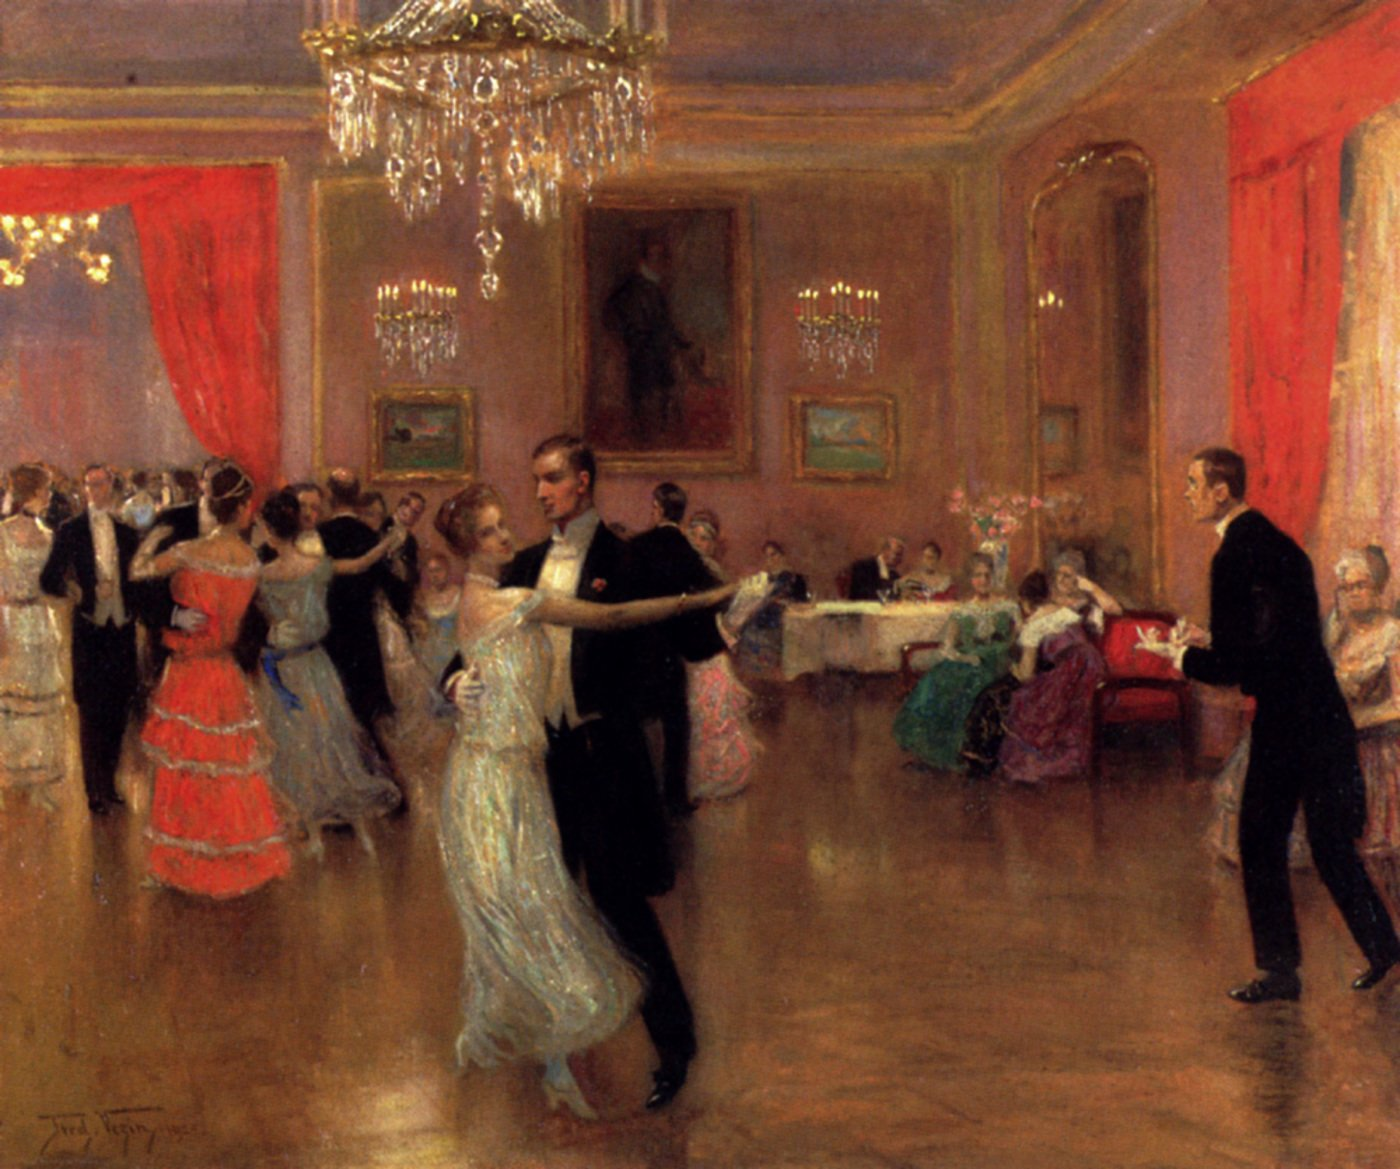
\includegraphics[width=0.7\textwidth]{theme.png}\\ % Тематическая картинка к танцвечеру
\end{center}
\ifthenelse{\isundefined{\mobile}}{
\newcommand{\DanceBackground}{\tikz[remember picture,overlay]{ % Фоновые изображения
\node[opacity=1] at (3, -2.7) {
\includegraphics[width=152.8pt,height=116.6pt]{images/frame corner lt.png}};
\node[opacity=1] at (18.5, -2.7) {
\includegraphics[width=151pt,height=123pt]{images/frame corner rt.png}};
\node[opacity=1] at (18.5, -25) {
\includegraphics[width=151.8pt,height=130.8pt]{images/frame corner rb.png}};
\node[opacity=1] at (3, -25) {
\includegraphics[width=152.8pt,height=135.6pt]{images/frame corner lb.png}};
}}
\SetBgOpacity{1.0}
\SetBgAngle{0.0}
\SetBgScale{1.0}
\SetBgPosition{current page.north west}
\SetBgContents{\DanceBackground}
}{
% Для мобильной версии используется однотонный бледно-жёлтый фон, который (по некоторым исследованиям) даёт меньшую нагрузку на глаза читателя.
\pagecolor[rgb]{1.0, 1.0, 0.953125}
}

\newpage
\renewcommand*\contentsname{\center{Схемы танцев}}
\thispagestyle{empty}
\tableofcontents
\newpage
\Large

% Interdance - команда, использующаяся для танца, который включен в программу, но не имеет описания схемы. В таком случае он будет отдельной строкой в тексте документа, и представляется отдельным пунктом в оглавлении.
\Interdance{Вальс}
% Пример схемы в виде расклада по счётам. В скобках приводится английский перевод названия танца, или его оригинальное название.
\PucksDeceit % КД Шалость Пака
% Пример схемы в виде расклада по тактам, с использованием иллюстраций и гиперссылок на внешние сайты / источники.
% Показательная ошибка - название танца осталось на текущей странице. Чтобы исправить, раскомментируйте следующую строку.
% \newpage
\FrenchQuadrille % Французская кадриль в каре
\newpage % Принудительное разделение на страницы
% Отдельные фигуры оформлены с использованием окружения minipage, что позволяет не заботиться о том, что одна фигура окажется на разных страницах. Однако из-за этого может возникать пустое пространство.
\Bat % Кадриль Летучая мышь
% Пример "маленького" танца. Схема такого танца должна целиком располагаться на одной странице.
\Shapelloise % Шапелуаз
% Пример правильного использования кавычек. Система вёрстки использует "кавычки-лапки" в качестве типографских символов, не стоит их использовать.
\Interdance{Вальсовый котильон <<Доверие>>}
\newpage
% Обычно части танца выделяются заголовком. В некоторых случаях используется окружение NCap, как в большом фигурном вальсе. Это необходимо для логического разделения таким образом, чтобы заполнить наибольшее пространство наименьшими смысловыми единицами.
\BigWaltz % Большой фигурный вальс
\Norwegian % Норвежский Круговой
% Пример шотландского контрданса. Каждый такой SCD снабжается диаграммой (рекомендуется Keith Rose's Diagrams) и схемой типа MiniCribs.
\ShiftingBobbins % Shifting Bobbins
\SCDReminder % Памятка по обозначениям SCD
\end{document}